\section{Signed matrices and the reflection contradiction}
\label{reflect:section}

We continue under the assumption that there is no finite win.  Thus the
price function of \cref{thm:prices}, the feedback and specialization laws,
and the pivot laws all apply.  We construct a real involution with a large
price and then use the orthogonal reflection in its positive eigenspace
to obtain incompatible price bounds.  All dimensions in the two
specializations below are fixed before either specialization is made.

\subsection{Signed bit operators with an exact price}

On one bit, set
\[
 C=\begin{pmatrix}0&0\\1&0\end{pmatrix},\qquad
 Z=\begin{pmatrix}1&0\\0&-1\end{pmatrix},\qquad
 X=\begin{pmatrix}0&1\\1&0\end{pmatrix}.
\]
For $m\geq 1$, define matrices on $m$ bits by
\begin{equation}
 D_1=C,\qquad
 D_{m+1}=C\otimes I_{2^m}+Z\otimes D_m
       =\begin{pmatrix}D_m&0\\ I_{2^m}&-D_m\end{pmatrix},
 \qquad T_m=I_{2^m}+D_m.
 \label{reflect:signed-recursion}
\end{equation}
The matrices $D_m$ are strictly lower triangular in lexicographic bit
order.  Squaring the displayed block matrix shows inductively that
$D_m^2=0$.  In particular, $T_m$ is invertible and
$T_m^{-1}=I_{2^m}-D_m$.

The signed tensor summands in this recursion have the standard
Jordan--Wigner creation-operator form, with tensor factors in the reverse
order of the convention in
\citet[Section~II.B, Equations~(10)--(11)]{seeleyRichardLove2012}.
Here the bits label ordinary matrix coordinates. The recursion above
and the price arguments below provide all identities needed for the
proof.

\begin{lemma}
\label{reflect:triangular-price}
For every integer $m\geq1$,
\[
 p(T_m)=m2^{m-1}.
\]
\end{lemma}

\begin{proof}
We have $T_1=U$, so $p(T_1)=1$.  Put $n=2^m$ and consider the transition
from input forms $x=(x_1,\ldots,x_{2n})$ to output forms $y=K_0x$, where
\[
 K_0=U\otimes T_m
     =\begin{pmatrix}T_m&0\\ T_m&T_m\end{pmatrix}.
\]
We shall exchange each bottom input form with the corresponding bottom
output form, using only the exact \emph{scalar} pivot law of
\cref{lem:scalar-pivot}.  Here is a determinant check for every
intermediate exchange.

For any subset $H\subseteq\{n+1,\ldots,2n\}$ of already exchanged
positions, keep the forms in their original index positions and set
\[
 u_i=\begin{cases}y_i&i\in H,\\x_i&i\notin H,\end{cases}
 \qquad
 v_i=\begin{cases}x_i&i\in H,\\y_i&i\notin H.\end{cases}
\]
Let $U_H,V_H$ be their coefficient matrices relative to $x$.
Simultaneously permuting rows and columns to put $H$ first gives
\[
 U_H\sim
 \begin{pmatrix}K_0[H,H]&K_0[H,H^c]\\0&I\end{pmatrix},\qquad
 V_H\sim
 \begin{pmatrix}I&0\\K_0[H^c,H]&K_0[H^c,H^c]\end{pmatrix}.
\]
The row and column permutation signs cancel.  Every principal submatrix
of the unit lower triangular matrix $K_0$ is unit lower triangular, so
\begin{equation}
 \det U_H=\det K_0[H,H]=1,
 \qquad
 \det V_H=\det K_0[H^c,H^c]=1.
 \label{reflect:mixed-minors}
\end{equation}
The empty principal minor, when it occurs, has determinant one.
Thus both lists are bases and their current transition
$Q_H=V_HU_H^{-1}$ has determinant one.

For the next index $j\notin H$ in the bottom half, replacing $u_j$ by
$v_j$ changes the input determinant by the factor $(Q_H)_{jj}$.
Replacing $v_j$ by $u_j$ changes the output determinant by
$(Q_H^{-1})_{jj}$.  Applying \eqref{reflect:mixed-minors} to $H$ and
$H\cup\{j\}$ therefore gives
\[
 (Q_H)_{jj}=\frac{\det U_{H\cup\{j\}}}{\det U_H}=1,
 \qquad
 (Q_H^{-1})_{jj}=\frac{\det V_{H\cup\{j\}}}{\det V_H}=1.
\]
Move position $j$ to the last port in both bases.  The scalar diagonal
block required for the pivot is consequently one; the determinant of
its complementary principal block is, by the cofactor identity,
\[
 \det Q_H\,(Q_H^{-1})_{jj}=1.
\]
Both hypotheses of \cref{lem:scalar-pivot} hold at every step, and each
exchange preserves the price exactly.

After all bottom positions have been exchanged, write the original
inputs as $(a,b)$ and the bottom output as $z=T_ma+T_mb$.
Solving gives $b=T_m^{-1}z-a$.  Thus the final transition, from $(a,z)$
to $(T_ma,b)$, is
\[
 \begin{pmatrix}T_m&0\\-I&T_m^{-1}\end{pmatrix}.
\]
Conjugating by $\diag(I,-I)$ changes the lower left block to $I$;
the result is $T_{m+1}$ by \eqref{reflect:signed-recursion}.
Monomial invariance and the tensor law now give
\[
 p(T_{m+1})=p(U\otimes T_m)=2^m+2p(T_m),
\]
which proves the formula by induction.
\end{proof}

Fix an integer $d\geq1$.  On $d+1$ bits, of width $N=2^{d+1}$, put
\begin{equation}
 \Gamma=X\otimes I_{2^d}+Z\otimes D_d
       =\begin{pmatrix}D_d&I\\I&-D_d\end{pmatrix}.
 \label{reflect:gamma}
\end{equation}
Since $D_d^2=0$, this is a real involution.  Its price is also exact:
\begin{equation}
 p(\Gamma)=\frac{dN}{2}.
 \label{reflect:gamma-price}
\end{equation}
To verify this, multiplication on the left by the monomial
$X\otimes I$ gives $I+(XZ)\otimes D_d$.
The recursion expands as
\[
 D_d=\sum_{i=1}^d
       Z^{\otimes(i-1)}\otimes C\otimes I_{2^{d-i}}.
\]
Each nonzero entry therefore changes exactly one bit from zero to one,
increasing Hamming weight by one.  Define the signed monomial $P$ to
act on the first bit by $(XZ)^{-|b|}$ when the last $d$ bits have value
$b$ and Hamming weight $|b|$.  On a transition of these last bits from
weight $j$ to weight $j+1$, conjugation by $P$ changes the first-bit
factor to
\[
 (XZ)^{-(j+1)}(XZ)(XZ)^j=I_2.
\]
It leaves the identity term unchanged.  Hence
\[
 P\bigl(I+(XZ)\otimes D_d\bigr)P^{-1}=I_2\otimes T_d,
\]
and \eqref{reflect:gamma-price} follows from
\cref{reflect:triangular-price} and the tensor law.

We next record a transpose symmetry.  Define the signed orthogonal
monomial
\begin{equation}
 J=\bigotimes_{i=1}^{d+1}(Z^{i-1}X).
 \label{reflect:j-definition}
\end{equation}
For its $i$th factor $H_i=Z^{i-1}X$, direct multiplication gives
\[
 H_i^{\mathsf T}=(-1)^{i-1}H_i,\qquad
 H_iZH_i^{-1}=-Z,\qquad
 H_iCH_i^{-1}=(-1)^{i-1}C^{\mathsf T}.
\]
The first-bit term of $\Gamma$ is $X\otimes I$ and is fixed by this
conjugation.  Every other term has the form
\[
 Z^{\otimes(i-1)}\otimes C\otimes I_{2^{d+1-i}},
 \qquad 2\leq i\leq d+1.
\]
The $i-1$ prefix signs and the sign from the $C$ factor cancel.  It
follows that
\begin{equation}
 J\Gamma J^{-1}=\Gamma^{\mathsf T},\qquad
 J^{\mathsf T}=(-1)^{d(d+1)/2}J.
 \label{reflect:transpose-symmetry}
\end{equation}

On width $w=N^2$, set
\begin{equation}
 M=\Gamma\otimes\Gamma,\qquad
 L=\Gamma\otimes I_N-I_N\otimes\Gamma,\qquad
 S=J\otimes J,\qquad A=SL.
 \label{reflect:large-operators}
\end{equation}
The matrix $S$ is a symmetric orthogonal monomial, so $S^{-1}=S$.
Equation~\eqref{reflect:transpose-symmetry} gives
$SLS^{-1}=L^{\mathsf T}$, and consequently
\[
 A^{\mathsf T}=L^{\mathsf T}S^{\mathsf T}=SL=A.
\]
In particular, $A$ is real symmetric.  Moreover,
\begin{equation}
 (\Gamma\otimes I_N)L=I_w-M,
 \qquad
 E:=\ker A=\ker L=\ker(I_w-M).
 \label{reflect:kernel}
\end{equation}
Thus $E$ is the positive eigenspace of the involution $M$.

We shall need a count of the supported unordered off-diagonal pairs
of $A$.  The first-bit flip in $\Gamma$ has $N$ nonzero entries, and
each of its other $d$ bit terms has $N/2$ nonzero entries.  Their
supports are disjoint, since they change different bits.  Thus
$\nnz(\Gamma)=(1+d/2)N$.
The supports of $\Gamma\otimes I_N$ and $I_N\otimes\Gamma$ are
also disjoint: they change a bit in different tensor factors.
Therefore
\[
 \nnz(L)=(d+2)w,\qquad \nnz(A)=(d+2)w.
\]
Symmetry makes every supported off-diagonal pair account for two
entries.  If $h$ is the number of such pairs, we have
\begin{equation}
 h\leq (d/2+1)w.
 \label{reflect:pair-count}
\end{equation}

Let $R$ be the orthogonal reflection in $E$. The rest of the argument
will establish the bounds
\[
 (d-4)w\leq p(R)\leq
 \left(\frac{3d}{4}+\frac72\right)w.
\]
They are incompatible when $d>30$.
The upper bound uses the description $E=\ker A$: a polynomial
perturbation has one dense pair factor of price at most $3/2$ for
each supported pair of $A$, at generic parameter values. Two algebraic
specializations turn this bound into a price for the reflection.
The lower bound uses $E$ as the positive eigenspace of $M$, whose
tensor price is $dw$.
Its graph description will recover the full price of $M$ from $R$, at
a cost of at most $4w$. Thus the contradiction comes from the different
coefficients of $d$, while the changes of boundary coordinates cost
only a fixed multiple of the width.

\subsection{Pricing a reflection by two algebraic specializations}

The following statement isolates the use of sparsity.  Orthogonality
refers to the usual real inner product; all real maps and subspaces
are then complexified when their prices are taken.

\begin{lemma}
\label{reflect:sparse-reflection}
Let $A$ be a real symmetric $w\times w$ matrix with $h$ supported
unordered off-diagonal pairs.  Let $R$ act as $+I$ on $\ker A$ and
as $-I$ on $(\ker A)^\perp$.  Then
\[
 p(R)\leq \frac32h+2w.
\]
\end{lemma}

\begin{proof}
Write $e_{ij}$ for matrix units, and fix any order of the supported
pairs.  Form the polynomial matrix
\begin{equation}
 K(\eps)=\left(I+\eps\diag(A_{11},\ldots,A_{ww})\right)
       \prod_{\substack{i<j\\A_{ij}\ne0}}
       \left(I+\eps A_{ij}(e_{ij}+e_{ji})\right).
 \label{reflect:polynomial-product}
\end{equation}
Then $K(0)=I$ and $K'(0)=A$.  Outside a finite set $E_0$,
the diagonal factor is an invertible monomial and every other factor
acts on its two coordinates as the dense invertible matrix
\[
 \begin{pmatrix}1&\eps A_{ij}\\\eps A_{ij}&1\end{pmatrix}.
\]
For example, $E_0$ may contain zero, the roots of the diagonal-factor
determinant, and all roots of $1-\eps^2A_{ij}^2$ for the supported
pairs.  These are finitely many roots of nonzero polynomials.
By \cref{lem:pair-price}, direct sums, and product subadditivity,
\begin{equation}
 p(K(\eps))\leq \frac32h\qquad(\eps\notin E_0).
 \label{reflect:product-price}
\end{equation}

Put $Q(\eps)=(K(\eps)-I)/\eps$, with its polynomial extension
$Q(0)=A$.  First fix a parameter $t$ outside the single finite set
\begin{equation}
 \mathcal E=\{0\}\cup
 \{\lambda^{-1},-\lambda^{-1}:
                    \lambda\in\operatorname{spec}(A),\ \lambda\ne0\}.
 \label{reflect:outer-exceptions}
\end{equation}
The polynomial matrices
\[
 C_+(\eps)=I+tQ(\eps),\qquad C_-(\eps)=I-tQ(\eps)
\]
have nonzero determinants at zero, since $I\pm tA$ are invertible.
Consequently the rational output
\[
 H_t(\eps)=C_+(\eps)C_-(\eps)^{-1}
\]
is regular and invertible at zero.

For this fixed $t$, exclude also $\eps=0,t,-t$ and the roots of
$\det C_+(\eps)\det C_-(\eps)$, in addition to $E_0$.
This defines a finite set $E_t$, which may depend on $t$.
For $\eps\notin E_t$ define
\[
 m=\frac{\eps-t}{\eps+t},\qquad
 s=\frac{t}{\eps+t},\qquad
 v=\frac{2\eps t}{(\eps+t)^2},
\]
and consider the data--state cell
\begin{equation}
 F_{t,\eps}=
 \begin{pmatrix}mI_w&K(\eps)\\vI_w&sK(\eps)\end{pmatrix}
 =\begin{pmatrix}mI_w&I_w\\vI_w&sI_w\end{pmatrix}
   \diag(I_w,K(\eps)).
 \label{reflect:feedback-cell}
\end{equation}
The first factor is a direct sum, after reordering, of $w$ scalar
pair matrices.  Their determinants are
\[
 ms-v=-\frac{t}{\eps+t}\ne0.
\]
Hence the cell is invertible.  Its direct block $mI_w$ is invertible,
and its feedback denominator at feedback parameter one satisfies
\begin{equation}
 I_w-sK(\eps)=\frac{\eps}{\eps+t}C_-(\eps),
 \label{reflect:feedback-denominator}
\end{equation}
so that denominator is invertible too.  Its feedback output is exactly
\begin{align*}
 mI_w+K(\eps)(I_w-sK(\eps))^{-1}v
 &=\bigl(mI_w+(v-ms)K(\eps)\bigr)
                         (I_w-sK(\eps))^{-1}\\
 &=C_+(\eps)C_-(\eps)^{-1}=H_t(\eps).
\end{align*}
The last equality follows from
$mI_w+(v-ms)K(\eps)=\eps C_+(\eps)/(\eps+t)$.
The output is invertible by the choice of $E_t$, so every hypothesis
of \cref{thm:feedback} is satisfied.

An invertible scalar pair has price at most two.  The factorization
\eqref{reflect:feedback-cell} and \eqref{reflect:product-price}
therefore imply
\[
 p(H_t(\eps))\leq p(F_{t,\eps})
              \leq p(K(\eps))+2w
              \leq \frac32h+2w
              \qquad(\eps\notin E_t).
\]
Apply \cref{thm:specialization} to the rational matrix $H_t$ at
$\eps=0$.  This proves
\begin{equation}
 p\bigl((I+tA)(I-tA)^{-1}\bigr)\leq C_A,
 \qquad C_A=\frac32h+2w,
 \qquad t\notin\mathcal E.
 \label{reflect:first-specialization}
\end{equation}
The quantifiers here are useful: $A,w,h$ and $C_A$ were fixed first;
for \emph{each} $t\notin\mathcal E$ there is a finite $E_t$ giving
the same bound, and specialization is applied separately for that
$t$.  Thus \eqref{reflect:first-specialization} holds for every
$t$ outside one finite set, with one price bound.
Only the rational output is specialized.  At $\eps=0$ the cell
itself would have $m=-1$, $s=1$, $v=0$, and $K=I$, making its
feedback denominator zero; no feedback law is applied to that cell.

For the second specialization use $z=1/t$ and the rational matrix
\[
 Y(z)=(zI_w+A)(zI_w-A)^{-1}.
\]
By the Real Spectral Theorem, $A=O\diag(\lambda_1,\ldots,\lambda_w)
O^{\mathsf T}$ for a real orthogonal $O$ and real eigenvalues
$\lambda_i$.  In this basis, the corresponding rational functions
are $(z+\lambda_i)/(z-\lambda_i)$.
If $\lambda_i=0$, this function is identically one after cancellation;
if $\lambda_i\ne0$, it is regular at zero with value minus one.
It follows that $Y$ is regular at zero and $Y(0)=R$, an invertible
matrix.  In particular, the zero eigenspace is semisimple; real
symmetry supplies exactly the diagonalizability needed for this
removable-singularity assertion.

For all $z$ outside
$\{0\}\cup\{\lambda,-\lambda:\lambda\in\operatorname{spec}(A),
\lambda\ne0\}$, we may take $t=1/z$ in
\eqref{reflect:first-specialization}.  Hence $p(Y(z))\leq C_A$
outside a finite set.  A second application of
\cref{thm:specialization} yields $p(R)\leq C_A$.
The orthogonal diagonalization was used to identify a rational
matrix and its value; it was not used as a priced implementation.
Neither specialization assumes continuity of $p$.
\end{proof}

Apply \cref{reflect:sparse-reflection} to $A=SL$ from
\eqref{reflect:large-operators}.  With $R$ the orthogonal reflection
in $E$ from \eqref{reflect:kernel}, \eqref{reflect:pair-count} gives
\begin{equation}
 p(R)\leq \frac32(d/2+1)w+2w
        =\left(\frac{3d}{4}+\frac72\right)w.
 \label{reflect:upper-bound}
\end{equation}

\subsection{The graph of the positive eigenspace}

Every nonzero term of $\Gamma$ changes exactly one bit, so $\Gamma$
anticommutes with the parity sign $\Pi=Z^{\otimes(d+1)}$.
Consequently $M$ anticommutes with $\Pi\otimes I_N$.
Order the coordinates according to this first-factor parity.
The two parts have equal width $r=w/2$, and in this order
\begin{equation}
 M=\begin{pmatrix}0&B\\B^{-1}&0\end{pmatrix}
 \quad\hbox{for some }B\in\GL_r(\R).
 \label{reflect:graph-involution}
\end{equation}
Indeed anticommutation forces the diagonal blocks to vanish, and
$M^2=I$ forces the two off-diagonal blocks to be mutual inverses.
The tensor law and \eqref{reflect:gamma-price} give
\begin{equation}
 p(M)=2N p(\Gamma)=dw=2p(B),
 \label{reflect:m-price}
\end{equation}
where the last equality follows by multiplying
\eqref{reflect:graph-involution} by a block-swap permutation and
then using direct sums and inverse symmetry.

Equation~\eqref{reflect:graph-involution} identifies
\[
 E=\{(Bv,v):v\in\R^r\},\qquad
 E^\perp=\{(u,v):B^{\mathsf T}u+v=0\}.
\]
Let $Q=I_r+B^{\mathsf T}B$.  For every nonzero real vector $v$,
$v^{\mathsf T}Qv=\|v\|^2+\|Bv\|^2>0$; hence $Q$ is invertible.
The columns of $\binom{B}{I_r}$ form a basis of $E$, so its
orthogonal projection is
\[
 P_E=\begin{pmatrix}B\\I_r\end{pmatrix}
       Q^{-1}\begin{pmatrix}B^{\mathsf T}&I_r\end{pmatrix}.
\]
As $R=2P_E-I_w$, its off-diagonal blocks in the parity order are
\begin{equation}
 R_{+,-}=2BQ^{-1},\qquad
 R_{-,+}=2Q^{-1}B^{\mathsf T}=R_{+,-}^{\mathsf T}.
 \label{reflect:invertible-offdiagonals}
\end{equation}
Both are invertible.  This use of positive definiteness is over
$\R$; all these invertible real matrices also define invertible
complex linear maps.

For $y=Rx$, order the input as $(x_-,x_+)$ and the output as
$(y_+,y_-)$.  The resulting transition is
\[
 K_R=\begin{pmatrix}R_{+,-}&R_{+,+}\\
                    R_{-,-}&R_{-,+}\end{pmatrix}.
\]
The two diagonal blocks required by \cref{lem:pivot-bound} are now
precisely the invertible blocks in
\eqref{reflect:invertible-offdiagonals}.
Pivot the second group of $r$ ports and then swap the two output
groups.  The resulting map
\[
 V:(x_-,y_-)\longmapsto(x_+,y_+)
\]
therefore satisfies
\begin{equation}
 p(V)\leq p(R)+4r.
 \label{reflect:graph-pivot-price}
\end{equation}

Since $R$ is the reflection in $E$, the vectors $x+y$ and $x-y$
belong to $E$ and $E^\perp$, respectively.  Their graph equations are
\[
 x_++y_+=B(x_-+y_-),\qquad
 x_+-y_+=-B^{-\mathsf T}(x_--y_-).
\]
For the invertible sum-and-difference map
\[
 F=\begin{pmatrix}I_r&I_r\\I_r&-I_r\end{pmatrix},
 \qquad F^{-1}=\tfrac12F,
\]
these equations state the exact identity
\begin{equation}
 FVF^{-1}=\diag(B,-B^{-\mathsf T}).
 \label{reflect:graph-diagonalization}
\end{equation}
The relation between the coordinates is displayed in
\cref{reflect:graph-figure}.

\begin{figure}[ht]
\centering
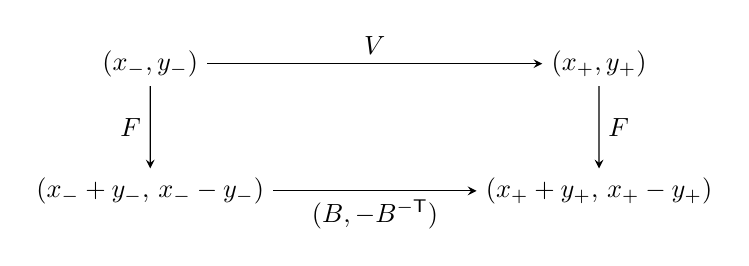
\begin{tikzpicture}[>=stealth, every node/.style={align=center},
                    scale=0.95, transform shape]
 \node (a) at (0,1.5) {$ (x_-,y_-) $};
 \node (b) at (6,1.5) {$ (x_+,y_+) $};
 \node (c) at (0,-0.2) {$ (x_-+y_-,\,x_--y_-) $};
 \node (e) at (6,-0.2) {$ (x_++y_+,\,x_+-y_+) $};
 \draw[->] (a) -- node[above] {$V$} (b);
 \draw[->] (a) -- node[left] {$F$} (c);
 \draw[->] (b) -- node[right] {$F$} (e);
 \draw[->] (c) -- node[below] {$\diag(B,-B^{-\mathsf T})$} (e);
\end{tikzpicture}
\caption{Pivoting the reflection exposes its two graph equations.
The sums are the parity components of $x+y\in E$; the differences
are the parity components of $x-y\in E^\perp$.
All four maps are exact invertible linear maps.}
\label{reflect:graph-figure}
\end{figure}

After interleaving coordinates, $F$ is a direct sum of $r$ invertible
scalar pair maps.  Thus $p(F)=p(F^{-1})\leq2r$.
Combining \eqref{reflect:m-price},
\eqref{reflect:graph-pivot-price}, and
\eqref{reflect:graph-diagonalization}, and using transpose and
inverse symmetry, yields
\begin{equation}
 dw=2p(B)
    =p\bigl(\diag(B,-B^{-\mathsf T})\bigr)
    \leq p(V)+4r
    \leq p(R)+8r
    =p(R)+4w.
 \label{reflect:lower-bound}
\end{equation}

\begin{theorem}[Existence of a finite win]
\label{thm:finite-win}
There exist an invertible nonmonomial matrix $A$ of a finite width
$q$, an integer $b\geq2$, and a word on exactly $q^b$ coordinates
implementing $A^{\otimes b}$ with monomials and fewer than
$bq^{b-1}$ calls to $A$.
\end{theorem}

\begin{proof}
If there were no finite win, the preceding construction and all its
price bounds would apply for every fixed integer $d\geq1$.
Equations~\eqref{reflect:upper-bound} and
\eqref{reflect:lower-bound} would imply
\[
 dw\leq\left(\frac{3d}{4}+\frac{15}{2}\right)w.
\]
Since $w>0$, this says $d\leq30$, contrary to choosing any fixed
integer $d>30$.  This contradiction proves the theorem.
\end{proof}

By \cref{prop:win-to-fourier}, the finite win of
\cref{thm:finite-win} supplies lengths $n_j\to\infty$ and exact
circuits in the stated scalar-gate model whose sizes $s_j$ satisfy
\[
 \frac{s_j}{n_j\log_2 n_j}\longrightarrow0.
\]
For every $c>0$ and every integer cutoff $n_0\geq2$, some $j$
therefore has $n_j\geq n_0$ and $s_j<c n_j\log_2 n_j$.
This proves the precise negative alternative in \cref{thm:main}.
The conclusion is nonuniform existence along an unbounded sequence;
the auxiliary price zero of monomials and the two specializations do
not alter the scalar gate costs or the exactness of those circuits.

